% ============================================================================
% COVER PAGE
% ============================================================================

\begin{center}

% Name
{\Huge\bfseries Juntang Wang}

\vspace{0.5em}

% Program & Affiliation
{\Large Duke Kunshan University \& Duke University}\\[0.3em]
{\large B.S. Applied Math \& Computational Science; Computer Science Track}\\[-0.2em]
{\small Class of 2026}

\vspace{1em}

% Contact Information
\begin{tabular}{c}
  \faIcon{envelope} \href{mailto:jw853@duke.edu}{jw853@duke.edu} \\[0.2em]
  \faIcon{github} \href{https://github.com/qqgjyx}{github.com/qqgjyx} \\[0.2em]
  \faIcon{globe} \href{https://www.qqgjyx.com}{www.qqgjyx.com} \\[0.2em]
  \faIcon{map-marker-alt} Kunshan, CN \textbullet{} Durham, USA
\end{tabular}

\vspace{1.5em}

% Two-column layout: Tagline + Headshot
\begin{minipage}[t]{0.6\textwidth}
  \raggedright
  \vspace{0pt}
  
  \textcolor{Accent}{\rule{\linewidth}{2pt}}
  
  \vspace{0.5em}
  
  {\large\textit{Bridging AI, mathematics, and biomedical modeling through computational design and visualization.}}
  
  % Epigraph (Marcus Aurelius) with adaptation summarizing work
  \vspace{0.8em}
  {\small\begin{quote}\itshape
  “The impediment to action advances action. What stands in the way becomes the way.”\\
  {\normalfont\textcolor{LightGray}{— Marcus Aurelius, Meditations 5.20}}\\[0.3em]
  \textcolor{TextGray}{Turning obstacles into methods across AI, math, and biomedicine.}
  \end{quote}}
  
  \vspace{0.35em}
  
  \textcolor{Accent}{\rule{\linewidth}{2pt}}
  
\end{minipage}\hfill
\begin{minipage}[t]{0.35\textwidth}
  \raggedleft
  \vspace{0pt}
  
  % Headshot
  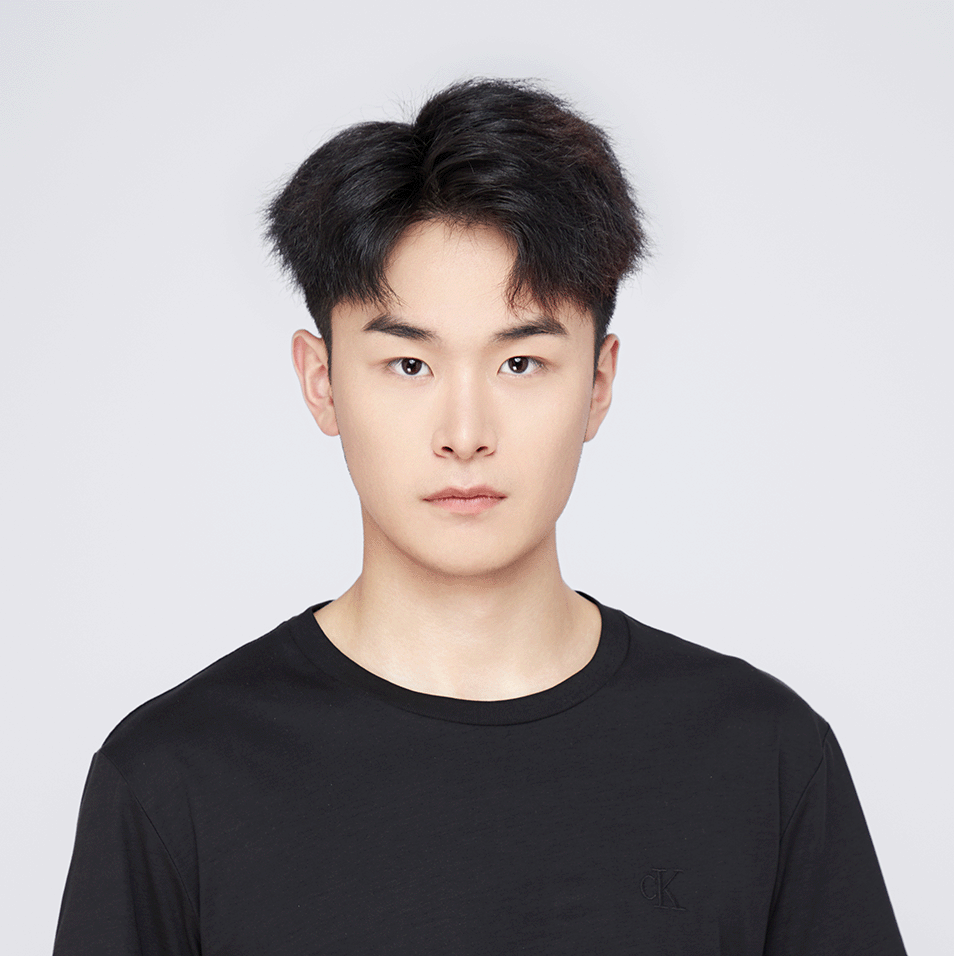
\includegraphics[width=0.76\linewidth]{assets/headshot.jpg}
  
  \vspace{0.5em}
  
  % QR code to website
  \qr{https://www.qqgjyx.com}
  
  \vspace{0.2em}
  
  {\footnotesize\textcolor{LightGray}{\textsc{Website}}}
\end{minipage}

\vspace{2.4em}

% Brief Introduction
\begin{minipage}{0.85\textwidth}
  \raggedright
  
  \section*{About This Portfolio}
  
  This portfolio showcases my work at the intersection of artificial intelligence, applied mathematics, and computational science. It includes research contributions under peer review at top-tier conferences (ICLR, BICS), open-source software tools with 600+ GitHub stars, teaching experience, and computational modeling projects.
  
  \vspace{0.5em}
  
  Each project demonstrates technical depth, practical impact, and creative problem-solving across machine learning, systems design, and computational modeling.
  
\end{minipage}

\end{center}

